\documentclass[11pt]{article}

% =========================
% PACKAGES
% =========================
\usepackage{amsmath, amssymb}
\usepackage{graphicx}
\usepackage{booktabs}
\usepackage{natbib}
\usepackage{geometry}
\usepackage{microtype}
\setlength{\emergencystretch}{3em}
\sloppy
\geometry{margin=1in}


% =========================
% TITLE
% =========================
\title{A Stochastic Temperature-Index Snowmelt Model for Probabilistic Runoff Estimation in a Himalayan Basin}
\author{Avinash Parla \\ Independent Researcher}
\date{}

\begin{document}
	
	\maketitle
	
	% =========================
\begin{abstract}
	Snowmelt-driven hydrological systems in high-mountain regions exhibit substantial variability due to complex terrain, spatial heterogeneity, and strong sensitivity to temperature. Conventional temperature-index models provide deterministic estimates that do not adequately capture this variability or the occurrence of extreme melt events.
	
	This study proposes a stochastic extension of the temperature-index snowmelt model that integrates state-dependent variability, autoregressive temporal persistence, and temperature-triggered jump processes. The framework is applied to the Chandra Basin in the western Himalayas using ERA5 reanalysis temperature data, SRTM-derived basin representation, and MODIS satellite-derived snow cover for independent validation.
	
	Monte Carlo simulations are employed to generate probabilistic estimates of snowmelt and runoff. Results show that while mean melt behavior remains consistent with deterministic estimates, stochastic formulations significantly enhance variability and produce heavy-tailed distributions, indicating an increased likelihood of extreme melt events. Sensitivity experiments further demonstrate that increasing persistence strengthens temporal memory, while higher jump probability increases the frequency and magnitude of extreme melt events without altering the overall seasonal structure.
	
	Validation against MODIS snow cover reveals that the deterministic model best captures seasonal timing (correlation $r = -0.698$), whereas stochastic models improve representation of melt magnitude and variability, achieving lower root mean square error (RMSE).
	
	The proposed framework provides a computationally efficient pathway for transitioning from deterministic snowmelt estimation to probabilistic hydrological modeling, with important implications for risk assessment, water resource management, and climate impact studies in snow-dominated regions.
\end{abstract}

\textbf{Keywords:} Snowmelt, Temperature-index model, Stochastic hydrology, Monte Carlo simulation, Uncertainty quantification, Himalayan basins
	% =========================
\section{Introduction}

Snow- and glacier-fed river systems play a critical role in sustaining water resources in high mountain regions, particularly across the Himalayas, where seasonal snowmelt contributes substantially to river discharge and downstream water availability \citep{Bookhagen2010, Immerzeel2010}. In many Himalayan basins, melt-driven flow dominates pre-monsoon hydrology, making accurate representation of snowmelt processes essential for understanding water availability and variability \citep{Singh2002, Barnett2005}.

Snowmelt has traditionally been modeled using deterministic approaches, most commonly through temperature-index (degree-day) formulations. These models establish a direct relationship between air temperature and melt rates and have been widely adopted due to their simplicity, robustness, and minimal data requirements \citep{Hock2003, Ohmura2001, Rango1995}. More physically detailed energy balance models explicitly account for radiative and turbulent fluxes governing melt processes, offering improved physical realism at the expense of increased data demands and computational complexity \citep{Marks1999, Essery2013}. Conceptual hydrological models such as HBV and SRM further integrate snowmelt into basin-scale runoff simulations, providing useful tools for operational forecasting and water resource assessment \citep{Bergstrom1976, Lindstrom1997, Martinec2008}.

Despite their widespread use, deterministic snowmelt models provide single-valued estimates of melt and runoff, implicitly assuming that the governing processes can be fully described through known relationships and parameters. In reality, snowmelt processes are inherently variable, influenced by spatial heterogeneity in snow distribution, elevation-dependent temperature gradients, and localized meteorological conditions \citep{Dozier2011, Essery2013}. These factors introduce variability that cannot be fully captured within deterministic frameworks, particularly in complex mountainous terrain.

To address uncertainty in hydrological systems, various stochastic and probabilistic approaches have been developed. These include ensemble modeling, stochastic perturbation of meteorological inputs, and probabilistic parameter estimation \citep{Montanari2007, Beven2001}. Monte Carlo methods are commonly used to propagate uncertainty through hydrological models, enabling estimation of output distributions and extreme events \citep{Koutsoyiannis2003, Robert2004}. However, in most existing approaches, uncertainty is introduced externally through inputs or parameters, while the underlying snowmelt model itself remains deterministic.

This separation between deterministic process representation and externally imposed uncertainty limits the ability of models to capture intrinsic variability arising from unresolved physical processes. In snow-dominated systems, variability is often strongly dependent on environmental conditions, particularly temperature, where small perturbations can lead to significant differences in melt rates during active ablation periods.

In this study, we propose a stochastic extension of the classical temperature-index snowmelt model in which variability is incorporated directly into the melt formulation. The approach represents melt as a combination of a deterministic component and a state-dependent stochastic term, allowing the model to generate a distribution of possible outcomes rather than a single estimate. Temporal persistence in variability is represented using an autoregressive process, while intermittent extreme melt events are captured through a temperature-triggered stochastic component.

The framework is applied to the Chandra Basin in the western Himalayas, a high-altitude, snow-dominated catchment where melt processes strongly influence seasonal hydrology. Using reanalysis-based temperature data and DEM-derived basin representation, the study aims to (i) implement a baseline deterministic snowmelt model, (ii) develop a stochastic formulation that captures condition-dependent variability, and (iii) quantify uncertainty in melt and runoff using Monte Carlo simulation.

By integrating deterministic modeling with internally generated stochastic variability, this work provides a pathway for transitioning from traditional snowmelt estimation toward probabilistic characterization of melt and runoff processes. Such an approach is particularly relevant for high-mountain regions, where variability and extremes play a critical role in hydrological response and water resource management. 

Unlike conventional approaches that introduce uncertainty externally through input perturbations or parameter ensembles, this study embeds stochastic variability directly within the snowmelt formulation, enabling intrinsic representation of process-level uncertainty and improving representation of variability and extremes.
	
	% =========================
\section{Study Area}

The study is conducted in the Chandra Basin, located in the western Himalayas within the Lahaul--Spiti region of Himachal Pradesh, India. The basin forms the upper catchment of the Chandra River, which originates from glaciated terrain near the Bara Shigri Glacier and later joins the Bhaga River to form the Chenab River system.

\begin{figure}[htbp]
	\centering
	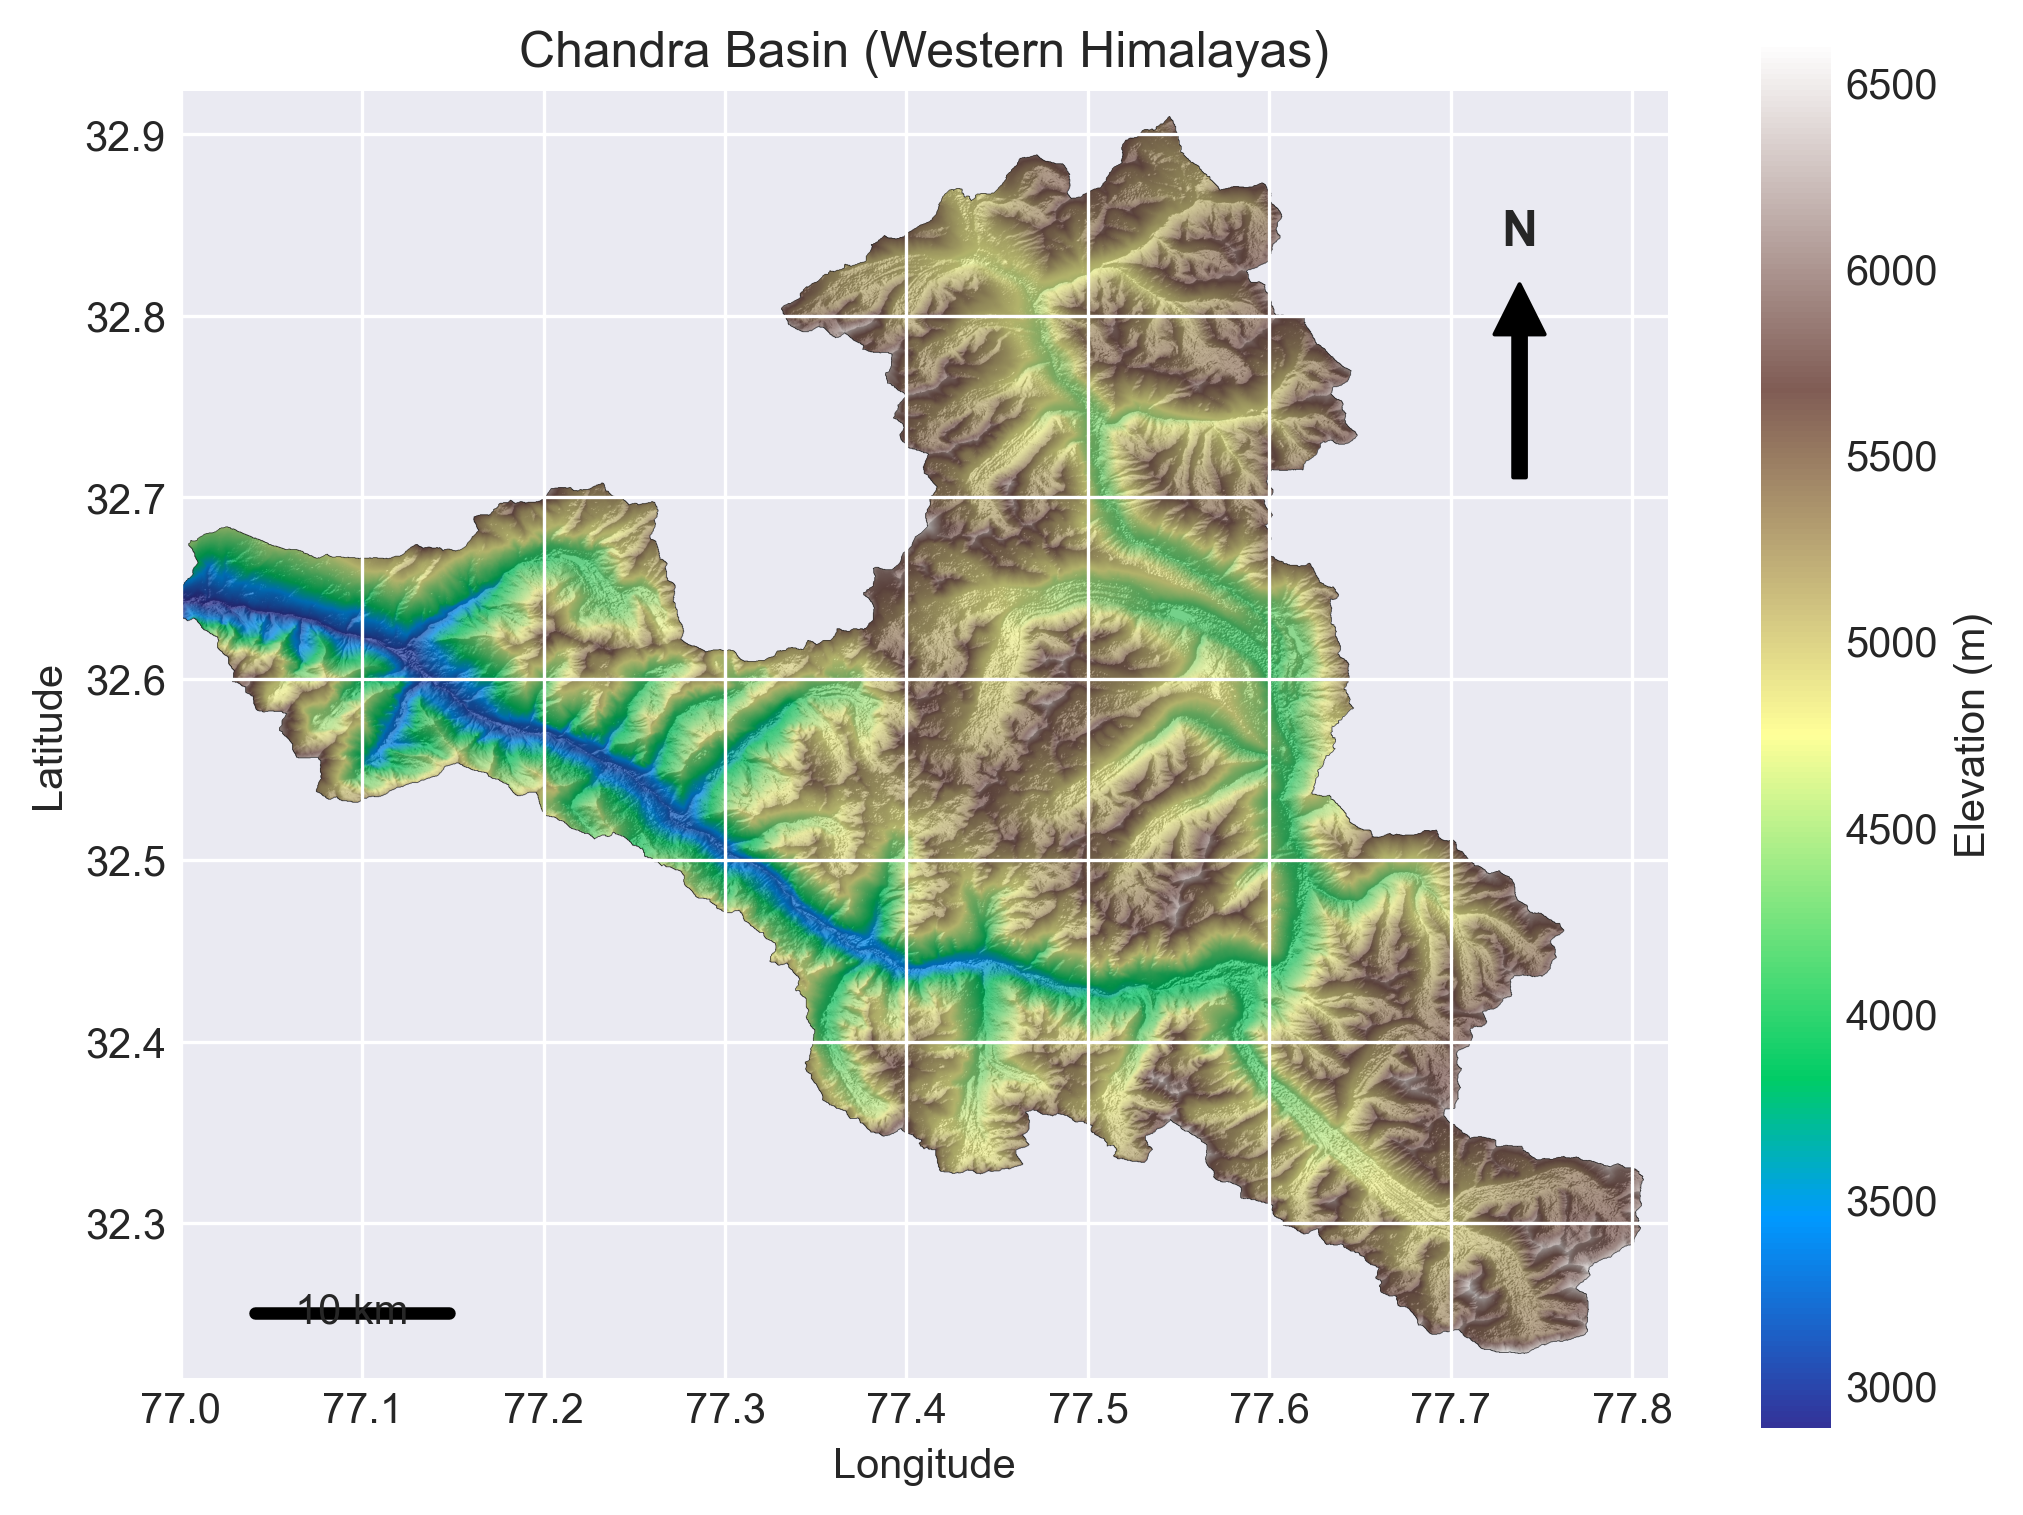
\includegraphics[width=0.75\textwidth]{../outputs/figures/figure_study_area_final.png}
	\caption{Topographic map of the Chandra Basin in the western Himalayas derived from SRTM DEM. Elevation is shown in meters above sea level with hillshade applied to enhance terrain features. The delineated basin boundary is overlaid in black, along with a north arrow and scale bar for spatial reference.}
	\label{fig:study_area}
\end{figure}

The basin is characterized by high-altitude mountainous terrain, with elevations ranging from approximately 3,000~m to over 6,000~m above sea level. This strong elevation gradient results in significant spatial variability in temperature, snow accumulation, and melt processes. The region experiences cold winters dominated by snowfall associated with western disturbances, leading to seasonal snowpack development.

During the pre-monsoon and early summer periods, rising temperatures drive snowmelt, which constitutes a major component of basin runoff. In contrast to monsoon-dominated regions, precipitation during summer is relatively limited, making melt processes the primary driver of hydrological response in the basin.

The terrain is highly complex, with steep slopes, varying aspects, and heterogeneous surface conditions, all of which influence the distribution and persistence of snow. Elevation-dependent temperature gradients and differential solar radiation further contribute to variability in melt rates across the basin.

Hydrologically, the basin is dominated by snow- and glacier-fed processes, with meltwater contributing significantly to streamflow in the Chandra River, a major tributary of the Chenab River system. The steep gradients, combined with pronounced elevation variability, lead to rapid runoff response and complex flow routing mechanisms.

For the purposes of this study, the basin is represented at an aggregated scale using a DEM-derived boundary and reanalysis-based meteorological forcing. While this approach does not explicitly resolve spatial heterogeneity, it allows for clear analysis of basin-scale melt dynamics and the development of a stochastic modeling framework.

A digital elevation model (DEM) derived from Shuttle Radar Topography Mission (SRTM) data was used for basin delineation and terrain analysis. The DEM provides sufficient spatial resolution to capture key geomorphological features influencing snow accumulation and melt processes. The spatial extent, elevation distribution, and terrain characteristics of the basin are shown in Figure~\ref{fig:study_area}.


	
	% =========================
\section{Data}

This study integrates reanalysis and topographic datasets to represent meteorological forcing and basin characteristics for the Chandra Basin. The selected datasets provide spatially consistent coverage and are suitable for high-altitude hydrological analysis.

\subsection{Meteorological Data}

Meteorological forcing is derived from the ERA5 reanalysis dataset produced by the European Centre for Medium-Range Weather Forecasts (ECMWF) \citep{Hersbach2020}. ERA5 provides globally consistent atmospheric variables by assimilating observations into a numerical weather prediction system.

In this study, daily near-surface air temperature (2 m temperature) is used as the primary driver of snowmelt. The ERA5 data are extracted over the spatial extent of the basin and processed to obtain basin-averaged temperature time series. Sub-daily data are aggregated to daily means to match the temporal resolution of the snowmelt model.

Temperature serves as the key input to the temperature-index formulation, capturing seasonal variations that drive snow accumulation and melt processes.

\subsection{Topographic Data and Basin Delineation}

Topographic characteristics of the basin are derived from the Shuttle Radar Topography Mission (SRTM) digital elevation model \citep{Farr2007}. The DEM is used to delineate the basin boundary and generate a spatial mask for extracting basin-specific meteorological data.

The delineation process involves hydrological conditioning of the DEM, including flow direction and flow accumulation analysis, followed by identification of the basin outlet and upstream contributing area. The resulting basin mask is then reprojected to match the coordinate system of the ERA5 dataset.

This mask is used to spatially aggregate meteorological variables, ensuring that all forcing data correspond strictly to the hydrological extent of the basin.

\subsection{Satellite-Derived Snow Cover Data}

Satellite-based snow cover observations are obtained from the Moderate Resolution Imaging Spectroradiometer (MODIS) daily snow product (MOD10A1, Collection 6.1) \citep{Hall2002}. This dataset provides global snow cover information at a spatial resolution of approximately 500~m. MODIS snow products have been widely used for large-scale snow cover monitoring due to their consistent temporal coverage and validated retrieval algorithms \citep{hall2019}.

For this study, MODIS snow cover data were accessed via Google Earth Engine and processed to extract basin-averaged snow fraction time series over the Chandra Basin. Pixels with valid Normalized Difference Snow Index (NDSI) values were retained, and quality-controlled observations were used to compute basin-averaged snow fraction time series.

Due to cloud contamination and classification uncertainty inherent in optical remote sensing, the MODIS dataset is not directly assimilated into the model, but used exclusively for independent validation of modeled snowmelt dynamics. To ensure temporal consistency, missing observations due to cloud contamination were implicitly handled through temporal smoothing, and the resulting snow fraction time series was used exclusively for validation purposes. The MODIS-derived snow fraction provides an independent observational constraint on snow depletion dynamics, enabling indirect validation of modeled melt processes.

\subsection{Data Processing and Basin Averaging}

All datasets are processed to ensure temporal and spatial consistency. The key steps include:

\begin{itemize}
	\item Reprojection of basin boundaries to match ERA5 grid coordinates
	\item Construction of a basin mask from DEM-derived polygons
	\item Extraction of grid points within the basin extent
	\item Computation of basin-averaged temperature time series
\end{itemize}

The modeling framework operates at a daily temporal resolution and uses spatially aggregated variables to focus on basin-scale dynamics. While this approach simplifies spatial heterogeneity, it provides a tractable framework for developing and evaluating stochastic extensions of snowmelt modeling.

The analysis period spans multiple years to capture repeated seasonal cycles of snow accumulation and melt, ensuring robust characterization of variability and extremes.


\section{Background: Snowmelt Modeling and Uncertainty}

Snowmelt modeling plays a central role in hydrological analysis of cold and high-altitude regions, where seasonal snow accumulation and ablation strongly influence runoff generation. Over the past decades, a range of modeling approaches have been developed, broadly categorized into empirical temperature-index models and physically based energy balance models.

Temperature-index models, also known as degree-day models, are among the most widely used approaches due to their simplicity and minimal data requirements. These models assume a linear relationship between air temperature and snowmelt, providing a computationally efficient approximation of melt processes \cite{Hock2003, Ohmura2001}. Despite their empirical nature, they have been successfully applied in mountainous regions where data availability is limited.

In contrast, energy balance models attempt to explicitly resolve the physical processes governing snowmelt, including radiative fluxes, sensible and latent heat exchange, and ground heat flux \cite{Marks1999, Essery2013}. While these models offer greater physical realism, they require detailed meteorological inputs and are computationally more demanding, limiting their applicability in data-scarce regions.

Conceptual and semi-distributed hydrological models, such as the HBV model and the Snowmelt Runoff Model (SRM), integrate simplified snowmelt formulations within broader runoff frameworks \cite{Bergstrom1976, Lindstrom1997, Martinec2008}. These models are widely used for basin-scale simulations but rely on calibrated parameters and simplified process representations.

Despite their widespread use, deterministic snowmelt models provide single-valued estimates of melt and runoff, implicitly assuming that system behavior can be fully described through known relationships and parameters. However, snow and cryospheric systems are inherently variable due to spatial heterogeneity, temporal variability in meteorological forcing, and unresolved sub-grid scale processes \cite{Dozier2011, Essery2013}.

To address these limitations, stochastic and probabilistic approaches have been introduced in hydrological modeling. Common methods include stochastic perturbation of meteorological inputs, ensemble simulations, and probabilistic parameter estimation \cite{Montanari2007, Beven2001}. Monte Carlo techniques are frequently used to propagate uncertainty and generate distributions of possible outcomes \cite{Koutsoyiannis2003}.

However, in most existing approaches, uncertainty is introduced externally through inputs or parameters, while the underlying snowmelt model remains deterministic. This separation limits the ability of models to represent intrinsic variability arising from unresolved physical processes.

In reality, snowmelt variability is often state-dependent, particularly near melting conditions where small perturbations in temperature or energy fluxes can lead to large differences in melt rates. This highlights the need for modeling frameworks that incorporate stochastic variability directly within the governing equations of snowmelt.

The present study addresses this gap by extending the classical temperature-index model through the inclusion of state-dependent stochastic components. By embedding variability within the melt formulation itself, the approach enables probabilistic characterization of snowmelt and runoff, providing a bridge between deterministic modeling and risk-based hydrological analysis.

	
	% =========================
	\section{Methodology}
	
	The modeling framework adopted in this study builds upon the classical temperature-index (degree-day) snowmelt formulation and extends it by incorporating stochastic variability to represent unresolved physical processes. The methodology consists of four main components: (i) deterministic snowmelt modeling, (ii) stochastic variability representation, (iii) runoff estimation, and (iv) probabilistic simulation using Monte Carlo methods.
	
	\subsection{Deterministic Snowmelt Model}
	
	Snowmelt is estimated using a temperature-index approach, which relates melt to air temperature above a threshold value:
	
	\begin{equation}
		M_t = \mathrm{DDF} \cdot \max(T_t - T_0, 0)
	\end{equation}
	
	where $M_t$ is the snowmelt at time $t$, $\mathrm{DDF}$ is the degree-day factor (mm~$^\circ$C$^{-1}$~day$^{-1}$), $T_t$ is basin-averaged air temperature, and $T_0$ is the threshold temperature, taken as $0^\circ$C.
	
	Temperature data are derived from ERA5 reanalysis and aggregated over the basin using a DEM-based spatial mask. The deterministic model provides a baseline estimate of melt driven solely by temperature.
	
	\subsection{Stochastic Snowmelt Formulation}
	
	To account for variability arising from unresolved processes such as spatial heterogeneity, sub-grid scale energy flux variability, and measurement uncertainty, a stochastic component is incorporated directly into the melt formulation:
	
	\begin{equation}
		M_t = M_t^{\mathrm{det}} + \sigma_t \, \epsilon_t
	\end{equation}
	
	where $M_t^{\mathrm{det}}$ is the deterministic melt, $\epsilon_t$ is a stochastic process, and $\sigma_t$ is a state-dependent scaling term controlling variability magnitude.
	
	This formulation allows the model to generate a distribution of melt outcomes rather than a single deterministic estimate.
	
	\subsection{Autoregressive Representation of Temporal Persistence}
	
	Temporal persistence in snowmelt variability is represented using a first-order autoregressive [AR(1)] process:
	
	\begin{equation}
		\epsilon_t = \phi \, \epsilon_{t-1} + \eta_t
	\end{equation}
	
	where $\phi$ is the persistence parameter ($0 < \phi < 1$), and $\eta_t \sim \mathcal{N}(0,1)$ is Gaussian white noise.
	
	This structure captures memory effects in melt processes, reflecting the influence of antecedent snowpack and atmospheric conditions.
	
	\subsection{State-Dependent Variability}
	
	The magnitude of stochastic variability is modeled as a function of melt conditions:
	
	\begin{equation}
		\sigma_t = a + b \cdot M_t^{\mathrm{det}}
	\end{equation}
	
	where $a$ and $b$ are empirical coefficients.
	
	This reflects the physical expectation that variability is low during cold conditions (no melt) and increases during active melt periods.
	
	\subsection{Temperature-Triggered Jump Process}
	
	To represent intermittent high-magnitude melt events, a temperature-dependent jump process is introduced. Jump occurrences are defined as:
	
	\begin{equation}
		J_t =
		\begin{cases}
			Z_t, & \text{if } T_t > T_c \text{ and } U_t < p \\
			0, & \text{otherwise}
		\end{cases}
	\end{equation}
	
	where $T_c$ is a critical temperature threshold, $U_t \sim \mathcal{U}(0,1)$ is a uniform random variable, $p$ is the probability of jump occurrence, and $Z_t$ is a random jump magnitude.
	
	The jump magnitude is modeled as a temperature-dependent stochastic variable, allowing stronger melt pulses under warmer conditions. This component captures episodic melt behavior that cannot be represented by smooth deterministic or autoregressive processes alone.
	
	The final stochastic process becomes:
	
	\begin{equation}
		\epsilon_t = \phi \, \epsilon_{t-1} + \eta_t + J_t
	\end{equation}
	
	\subsection{Parameter Selection and Sensitivity}
	
	The stochastic snowmelt model introduces several parameters that govern variability, persistence, and extreme event behavior. These include the autoregressive persistence coefficient ($\phi$), the state-dependent variability parameters ($a$, $b$), the probability of temperature-triggered jumps ($p$), and the critical temperature threshold ($T_c$).
	
	Parameter values are selected based on physical reasoning and exploratory analysis. The persistence parameter $\phi$ controls the memory of the stochastic process and is chosen within the range $0 < \phi < 1$ to ensure stability while capturing temporal correlation in melt variability. Higher values of $\phi$ produce smoother time series with stronger persistence, whereas lower values result in more rapidly fluctuating melt behavior.
	
	The variability parameters $a$ and $b$ define the magnitude of stochastic noise as a function of melt conditions. This formulation allows variability to increase during high melt periods, reflecting enhanced sensitivity to atmospheric forcing and surface processes. Parameter values are selected to ensure realistic variability without producing non-physical melt magnitudes.
	
	The jump probability $p$ and threshold temperature $T_c$ control the occurrence of episodic melt events. These parameters are chosen to represent rare but significant increases in melt during warm conditions, consistent with observed rapid snow depletion events.
	
	To provide quantitative insight into parameter influence, a targeted sensitivity experiment was conducted by systematically varying the persistence parameter ($\phi$) and jump probability ($p$) across representative ranges, while keeping all other parameters fixed. Specifically, $\phi$ was varied between 0.3 and 0.9 to assess changes in temporal persistence, and $p$ was varied between 0.05 and 0.3 to evaluate the frequency of temperature-triggered melt events. 
	
	For each parameter setting, the stochastic model was simulated over the full study period, and resulting melt time series were compared against the deterministic baseline. The resulting changes in melt dynamics are analyzed in the Results section, allowing assessment of how stochastic parameters influence variability, temporal structure, and extreme melt behavior. 
	
	All sensitivity experiments were performed using identical meteorological forcing and initial conditions, ensuring that observed differences arise solely from parameter variation.
	
	
	\subsection{Runoff Estimation}
	
	Snowmelt is converted to runoff using a linear transformation:
	
	\begin{equation}
		Q_t = k \cdot M_t
	\end{equation}
	
	where $Q_t$ is runoff and $k$ is a runoff coefficient representing basin-scale hydrological response.
	
	While simplified, this approach enables consistent comparison between deterministic and stochastic melt dynamics at the basin scale.
	
	\subsection{Monte Carlo Simulation Framework}
	
	Uncertainty in snowmelt and runoff is quantified using Monte Carlo simulation. Multiple realizations of the stochastic model are generated by sampling the stochastic components:
	
	\begin{equation}
		\eta_t \sim \mathcal{N}(0,1)
	\end{equation}
	
	Each realization produces a time series of melt and runoff, resulting in an ensemble of possible outcomes. Statistical measures such as mean behavior, variance, and extreme quantiles (e.g., 90th and 99th percentiles) are derived from the ensemble.
	
	This framework enables transition from deterministic prediction to probabilistic characterization of snowmelt and runoff processes.
	
	\subsection{Summary of Model Structure}
	
	The proposed framework extends the classical temperature-index model by integrating:
	
	\begin{itemize}
		\item State-dependent stochastic variability
		\item Temporal persistence via autoregressive processes
		\item Temperature-triggered jump dynamics
		\item Monte Carlo-based uncertainty quantification
	\end{itemize}
	
	By embedding stochasticity directly within the melt formulation, the model captures intrinsic variability in snowmelt processes rather than relying solely on external uncertainty inputs. This provides a more realistic representation of melt dynamics in complex mountainous environments.
	
	\subsection{Validation Framework}
	
	Model outputs are evaluated against satellite-derived snow cover observations to assess their ability to reproduce real-world snow dynamics. Since the model simulates melt while MODIS provides snow cover fraction, a direct comparison is not possible. Instead, a normalized comparison framework is adopted.
	
	Modeled melt time series are normalized to the range [0,1] to represent relative melt intensity, while MODIS snow fraction is smoothed using a rolling mean to reduce noise and cloud-related variability. Since snow cover decreases as melt increases, an inverse relationship between MODIS snow fraction and modeled melt is expected. This physical linkage forms the basis for model validation.
	
	Model performance is quantified using Pearson correlation coefficient and root mean square error (RMSE). Correlation assesses the ability of the model to reproduce seasonal timing of snow depletion, while RMSE evaluates agreement in magnitude and variability.
	
	This validation framework enables a physically consistent comparison between modeled melt dynamics and observed snow cover evolution, linking temperature-driven melt processes with satellite-derived snow depletion patterns.
	
	% =========================
\section{Results}

The proposed stochastic snowmelt framework is evaluated by comparing deterministic and stochastic model outputs, analyzing ensemble-based uncertainty, and examining the statistical characteristics of melt and runoff.

\subsection{Temporal Dynamics of Snowmelt}


Figure~\ref{fig:model_comparison} illustrates the temporal evolution of snowmelt simulated using the deterministic model, the AR(1)-based stochastic model, and the temperature-triggered jump model.


The deterministic model produces smooth seasonal melt cycles driven solely by temperature variations. The AR(1) model introduces temporal persistence, resulting in realistic short-term fluctuations around the deterministic baseline. The temperature-triggered jump model further enhances variability by generating intermittent high-magnitude melt events during warm conditions.

These results demonstrate that stochastic formulations capture both continuous variability and abrupt melt responses, which are not represented in traditional deterministic approaches.

\begin{figure}[htbp]
	\centering
	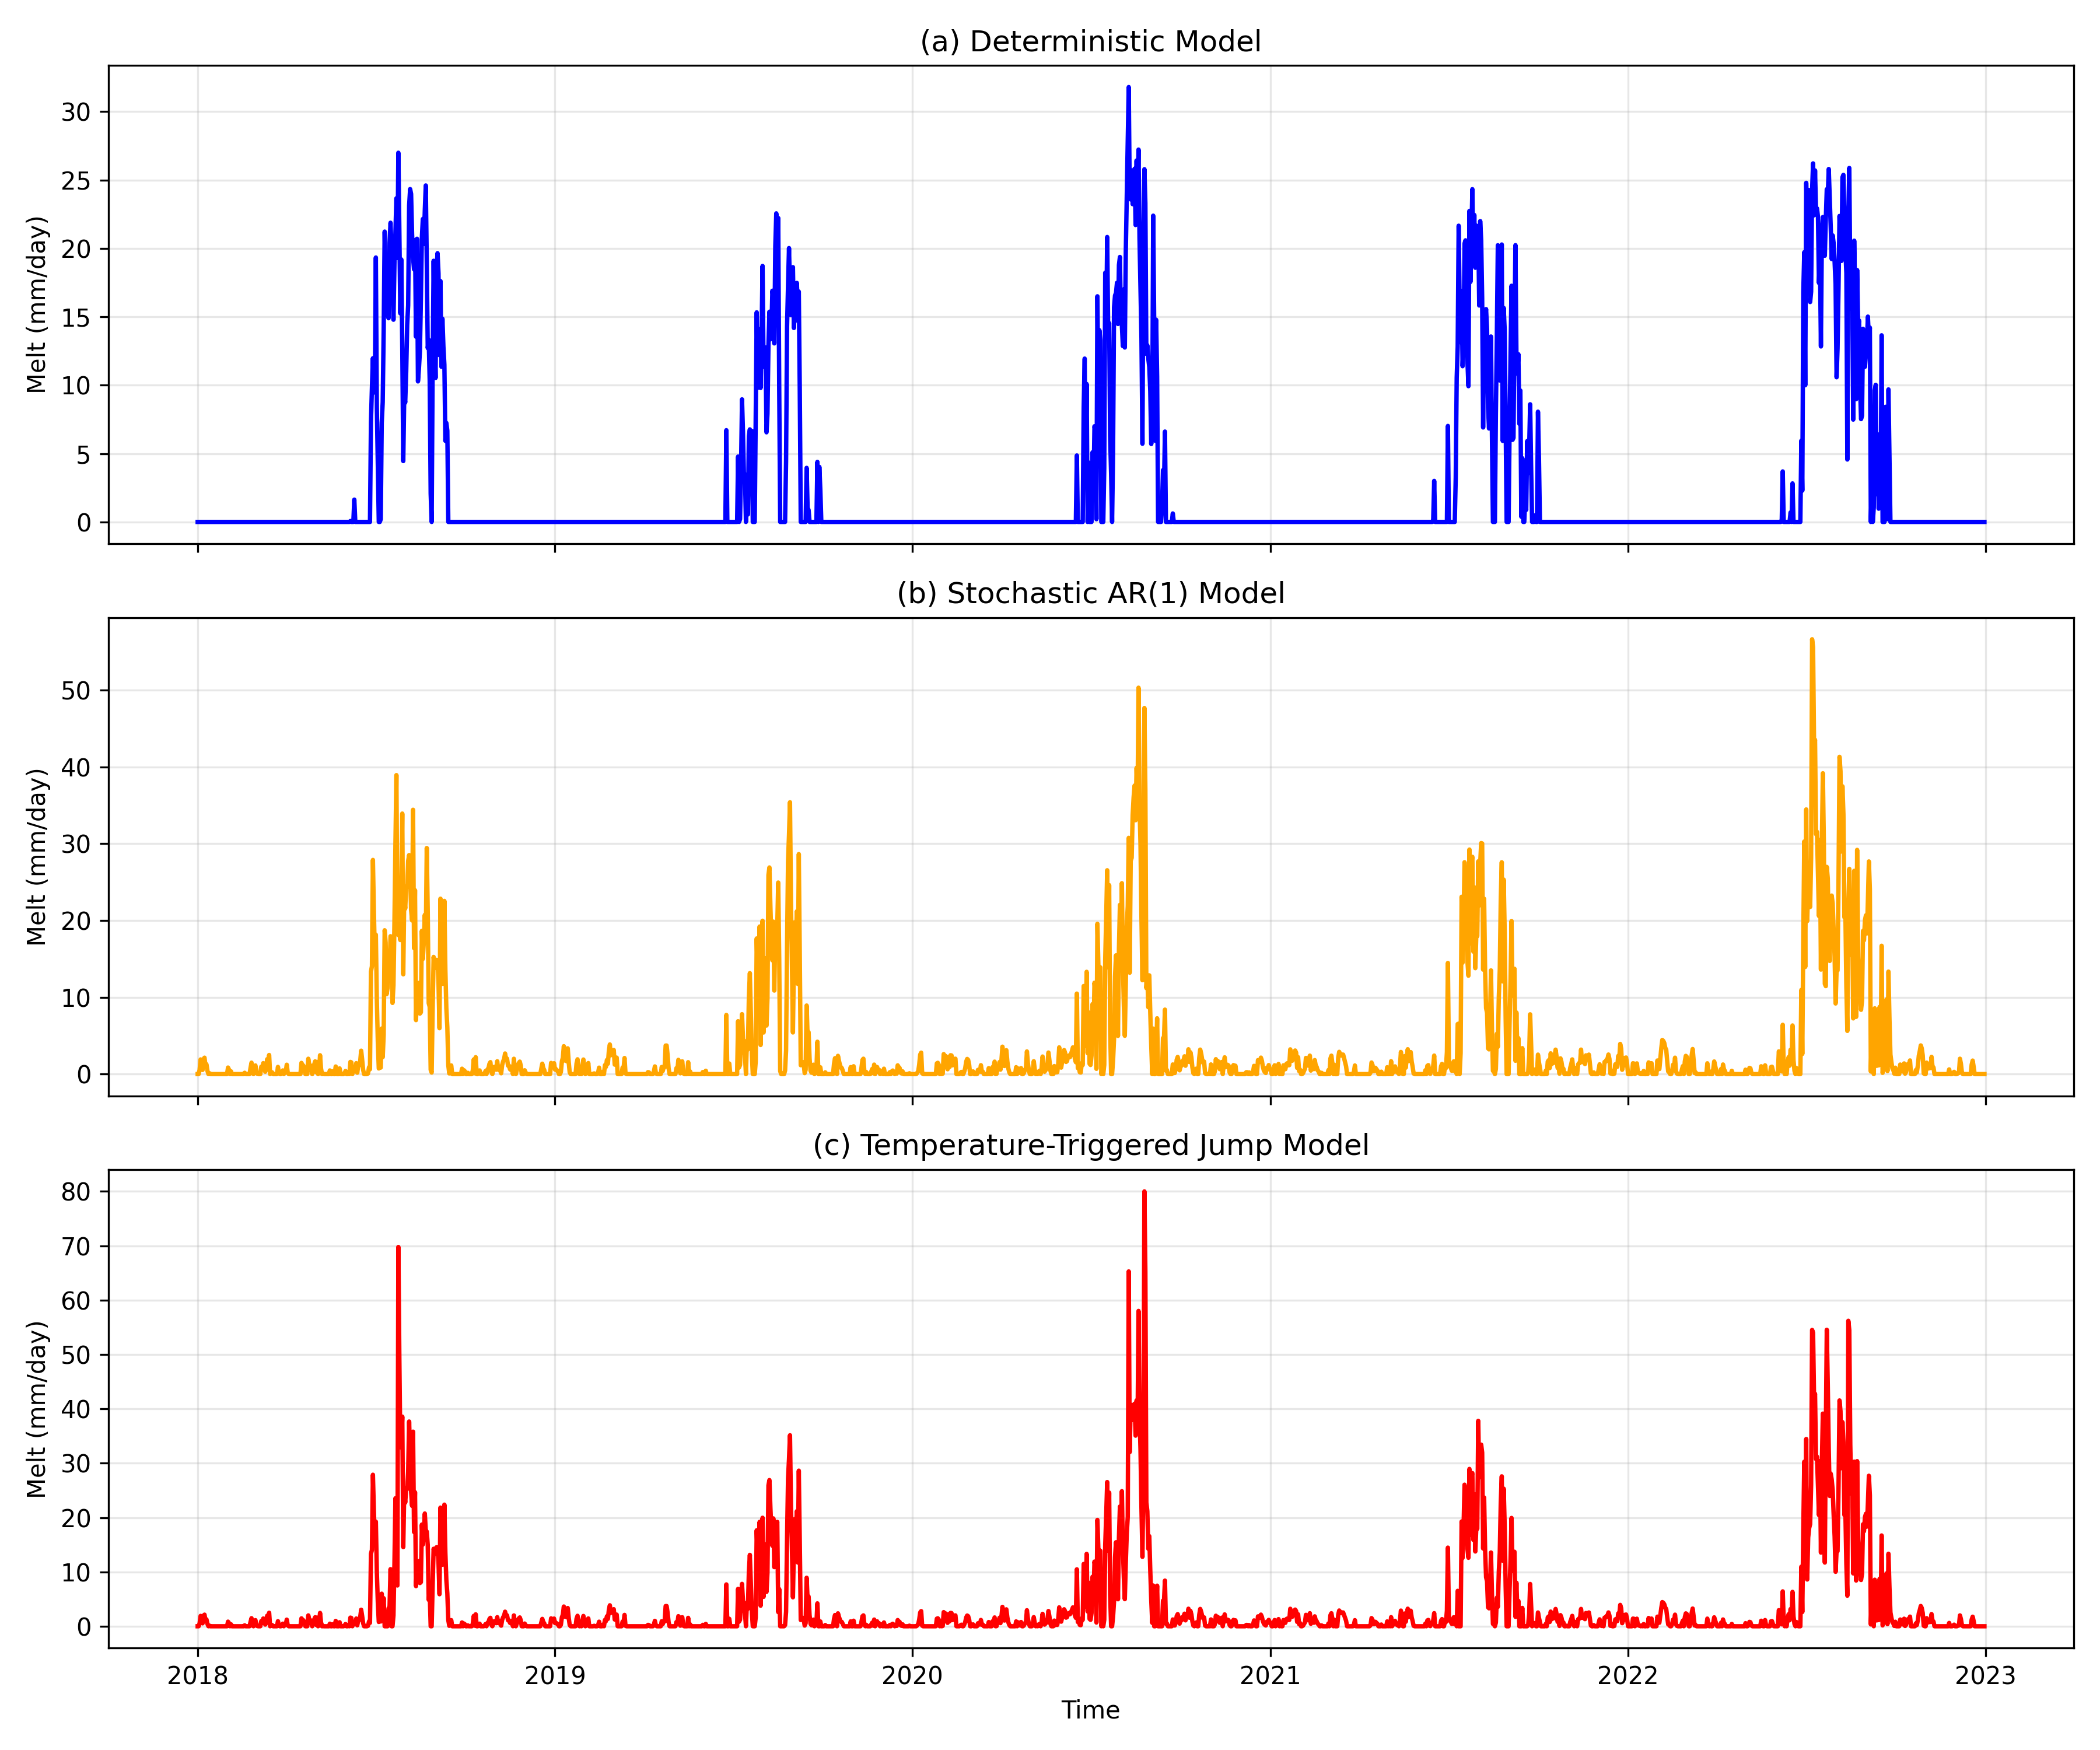
\includegraphics[width=0.85\textwidth]{../outputs/figures/figure_model_comparison.png}
	\caption{Temporal evolution of snowmelt for deterministic and stochastic models. The deterministic model produces smooth seasonal melt cycles, while the AR(1) model introduces persistent variability and the temperature-triggered jump model captures intermittent high-magnitude melt events.}
	\label{fig:model_comparison}
\end{figure}

\subsection{Uncertainty in Snowmelt Estimates}

Uncertainty is quantified using Monte Carlo simulation, generating an ensemble of possible melt realizations.

\begin{figure}[htbp]
	\centering
	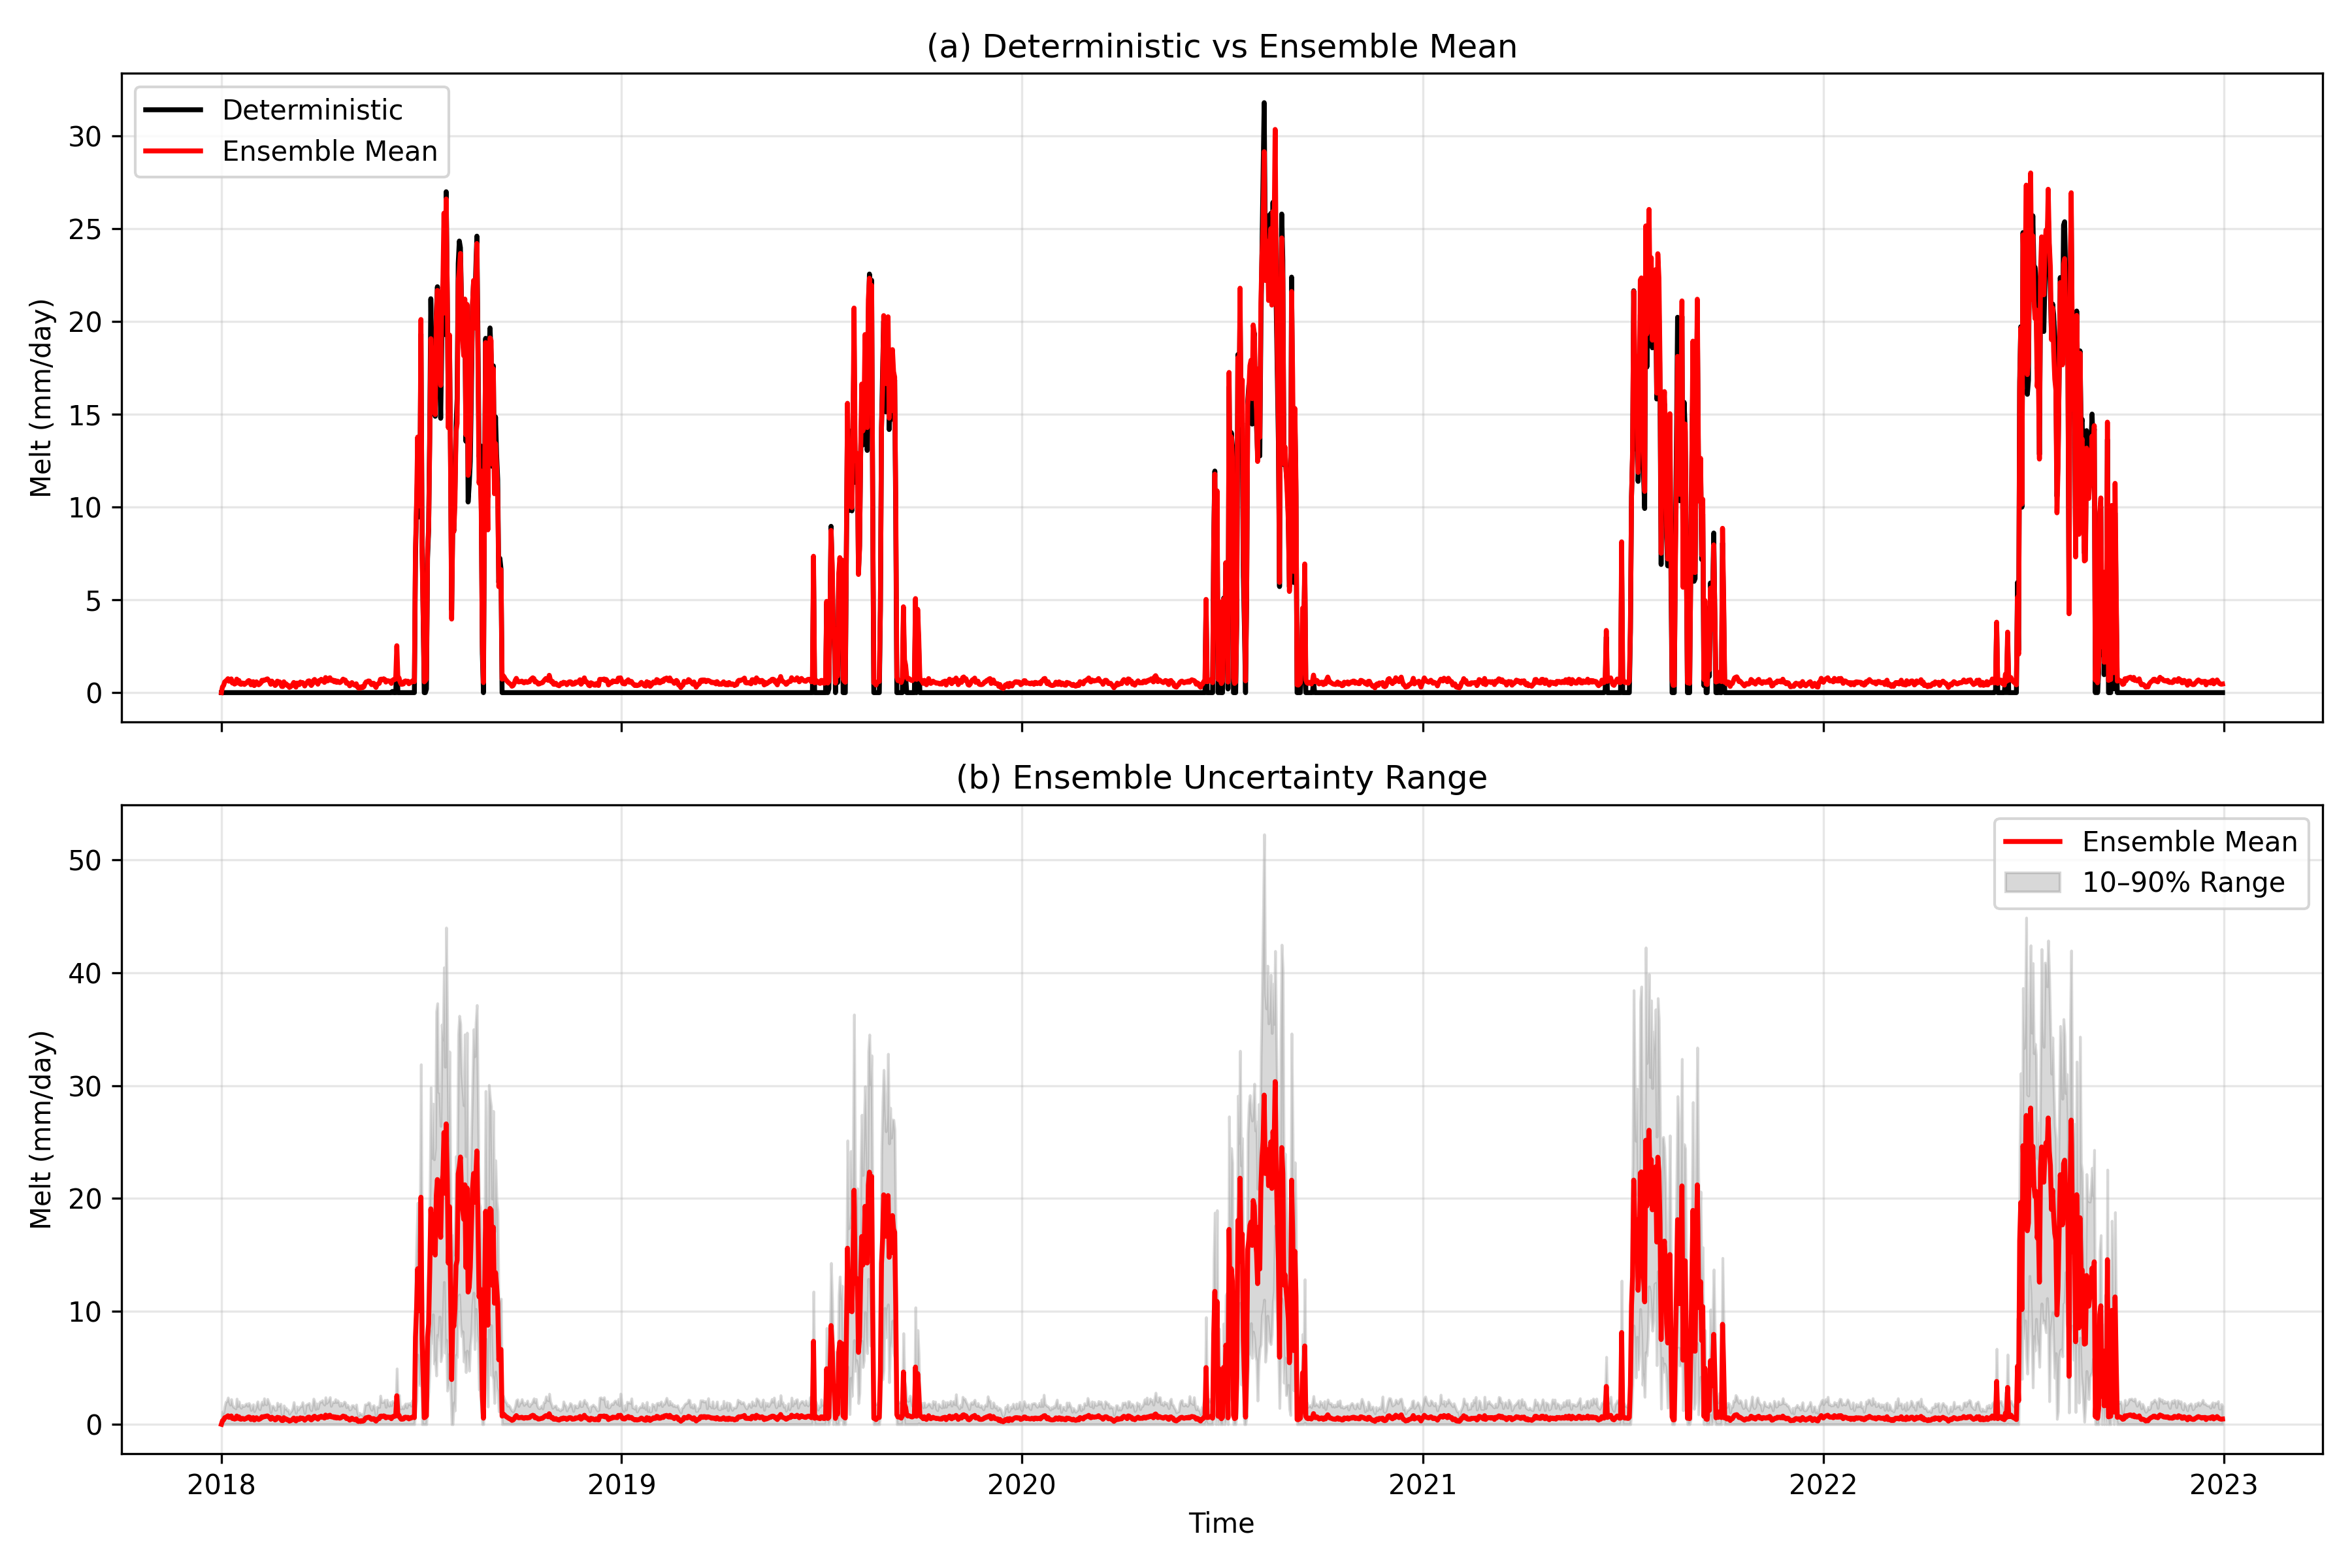
\includegraphics[width=0.85\textwidth]{../outputs/figures/figure_1_uncertainty.png}
	\caption{Snowmelt uncertainty derived from Monte Carlo simulation. The shaded region represents the 10-90\% ensemble range, which widens significantly during active melt periods, indicating strong state-dependent variability. The ensemble mean closely follows the deterministic estimate.}
	\label{fig:uncertainty}
\end{figure}

As shown in Figure~\ref{fig:uncertainty}, uncertainty is strongly state-dependent. During cold periods, melt remains close to zero with minimal variability. In contrast, during active melt periods, the uncertainty band widens significantly, reflecting increased sensitivity to stochastic perturbations.

\begin{figure}[htbp]
	\centering
	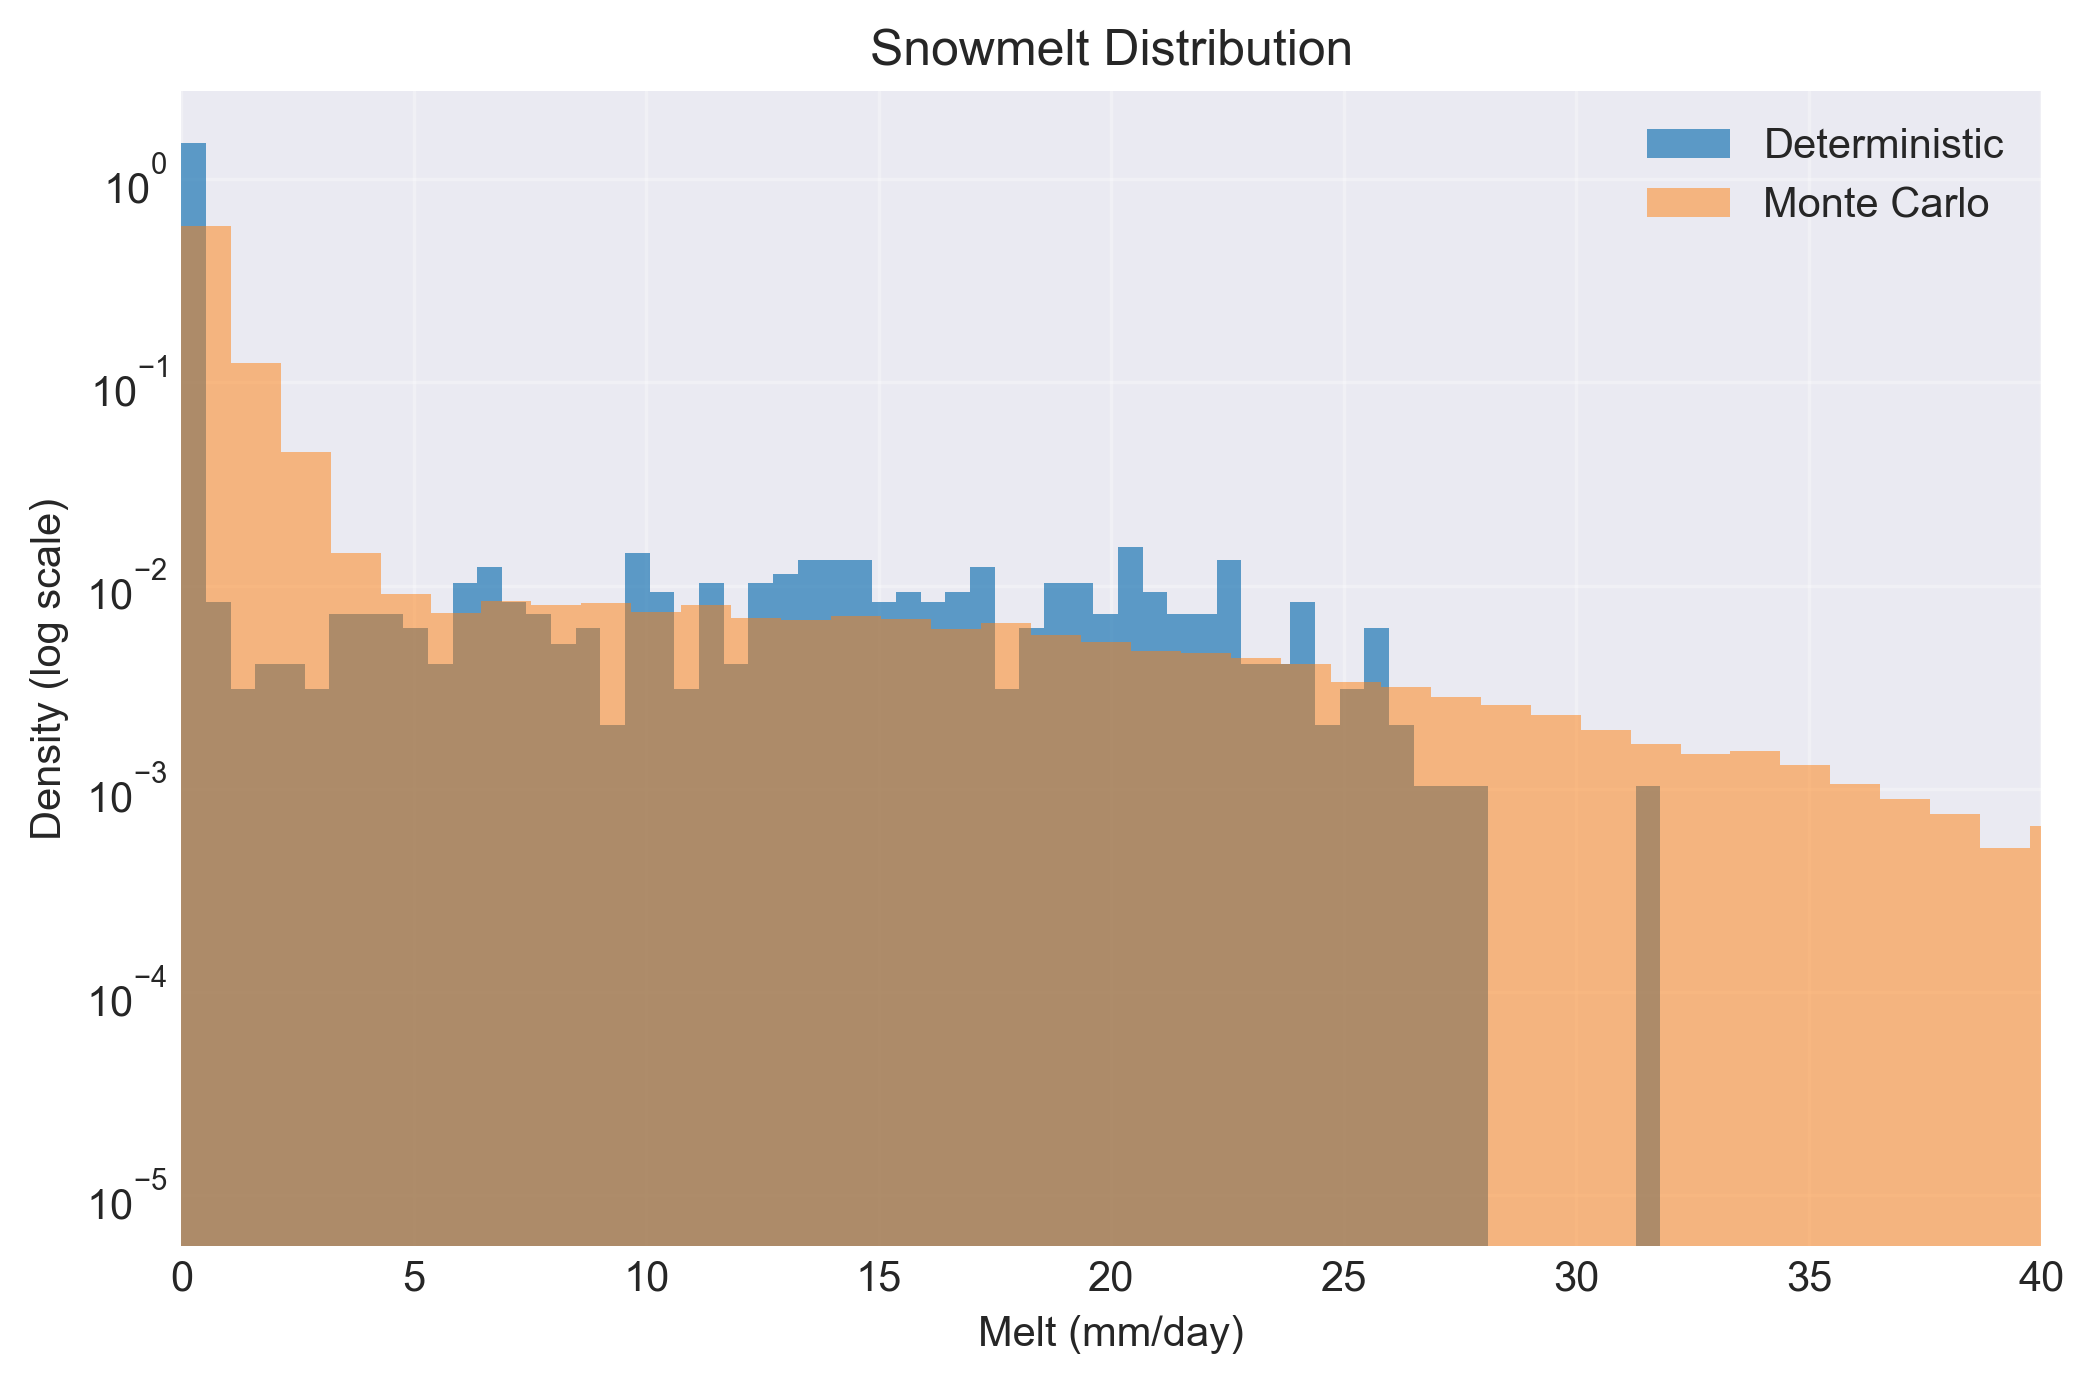
\includegraphics[width=0.75\textwidth]{../outputs/figures/figure_2_distribution.png}
	\caption{Distribution of snowmelt values on a logarithmic density scale. The stochastic model exhibits a broader distribution with a pronounced heavy tail, indicating an increased likelihood of extreme melt events compared to the deterministic formulation.}
	\label{fig:distribution}
\end{figure}

\subsection{Distribution of Snowmelt}

The distribution of snowmelt values is presented in Figure~\ref{fig:distribution}, comparing deterministic and stochastic simulations on a logarithmic density scale.

Both models exhibit high frequency near low melt values; however, the stochastic model produces a substantially broader distribution with a pronounced heavy tail. This indicates an increased probability of moderate and extreme melt events compared to the deterministic formulation.

The heavy tail behavior arises from the combined influence of autoregressive variability and temperature-triggered jumps, which amplify melt responses during favorable thermal conditions.

\subsection{Statistical Characteristics of Melt and Runoff}

Table~\ref{tab:stats} summarizes key statistical metrics for melt and runoff across model configurations.

\begin{table}[htbp]
	\centering
	\caption{Statistical summary of melt and runoff across deterministic and stochastic models.}
	\label{tab:stats}
	\begin{tabular}{lccccc}
		\hline
		Model & Mean & Std Dev & Max & P90 & P95 \\
		\hline
		Melt - Deterministic & 2.69 & 6.36 & 31.80 & 14.16 & 19.44 \\
		Melt - AR1 & 2.63 & 7.68 & 56.60 & 14.06 & 22.09 \\
		Melt - Temp Jump & 3.79 & 8.72 & 80.00 & 13.95 & 23.36 \\
		Runoff - Deterministic & 1.96 & 4.45 & 22.26 & 9.91 & 13.61 \\
		Runoff - AR1 & 2.54 & 5.37 & 39.62 & 9.84 & 15.41 \\
		Runoff - Temp Jump & 2.66 & 6.10 & 56.00 & 9.76 & 16.35 \\
		\hline
	\end{tabular}
\end{table}

This highlights the importance of incorporating stochastic processes when assessing hydrological extremes, particularly in snow-dominated basins. The stochastic models exhibit substantially higher variability and extreme values compared to the deterministic model. In particular, the temperature-triggered jump model produces the largest maximum melt and runoff values, highlighting its ability to represent extreme melt events.

\subsection{Parameter Sensitivity Analysis}

Figure 5 presents the results of the sensitivity experiments described in Section 5.6. 

A controlled sensitivity experiment was conducted to evaluate the influence of key stochastic parameters on model behavior. The persistence parameter ($\phi$) and jump probability ($p$) were varied across representative ranges while keeping other parameters constant. 

Figure~\ref{fig:sensitivity} shows that increasing $\phi$ results in smoother melt time series with stronger temporal persistence, while lower values produce more rapidly fluctuating behavior. This reflects the role of $\phi$ in controlling memory within the stochastic process. Notably, higher $\phi$ values also lead to more sustained melt events during peak periods.

Similarly, increasing the jump probability $p$ leads to more frequent high-magnitude melt events, significantly enhancing variability and extremes. Lower values of $p$ result in behavior closer to the deterministic baseline, while higher values produce frequent spikes that may exceed physically realistic melt rates.

Importantly, variations in both parameters primarily affect short-term variability and extreme behavior, while the  seasonal structure of melt remains largely unchanged. This suggests that the stochastic framework preserves the dominant temperature-driven signal while providing flexibility to represent uncertainty and variability.

These results indicate that model behavior is sensitive to parameter selection, but remains physically interpretable across a reasonable parameter range. This suggests that stochastic parameters primarily control higher-order statistics (variance and extremes) rather than first-order seasonal trends.

\begin{figure}[htbp]
	\centering
	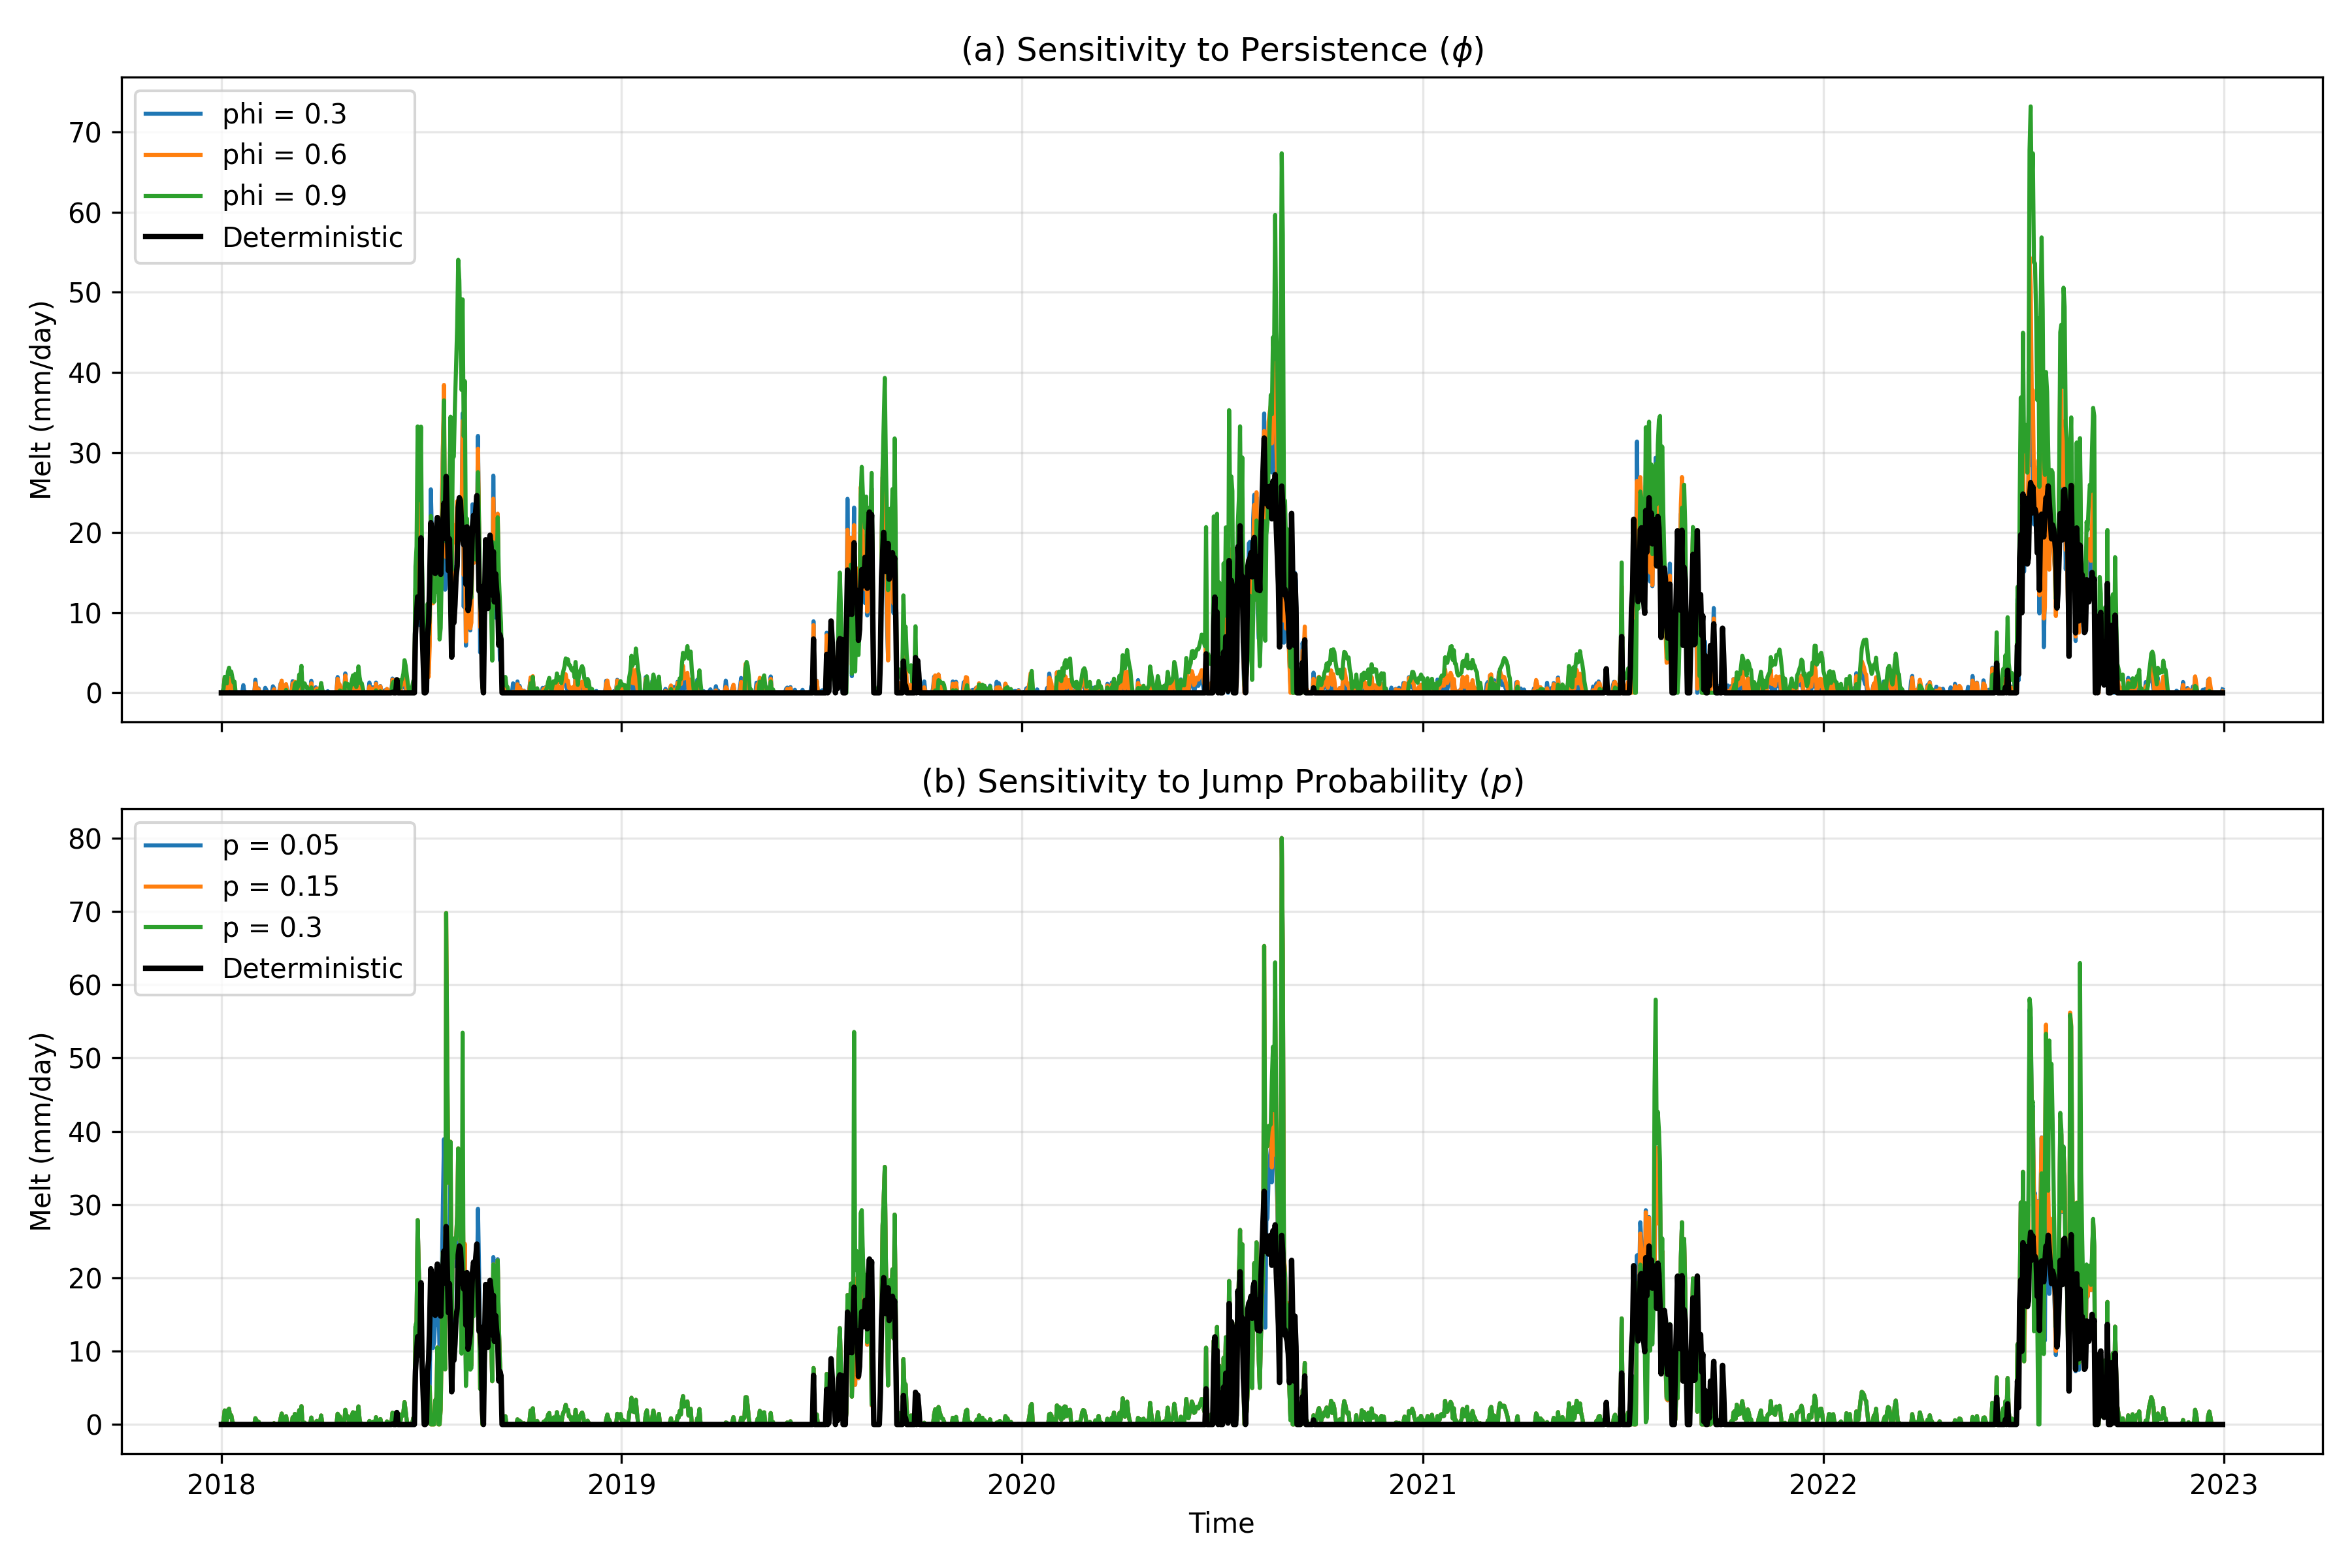
\includegraphics[width=\textwidth]{../outputs/figures/figure_sensitivity.png}
	\caption{Sensitivity of modeled snowmelt to key stochastic parameters. (a) Increasing persistence $\phi$ enhances temporal smoothness and memory in melt dynamics. (b) Increasing jump probability $p$ increases the frequency and magnitude of extreme melt events. The overall seasonal structure remains largely unchanged across parameter values.}
	\label{fig:sensitivity}
\end{figure}

\subsection{Summary of Model Behavior}

Overall, the results demonstrate that the proposed stochastic framework effectively extends the classical temperature-index model by capturing both variability and extreme melt behavior. The autoregressive component introduces realistic temporal persistence, while the jump process enables representation of episodic high-intensity melt events.

This combined approach provides a more comprehensive representation of snowmelt dynamics in complex mountainous environments.

\subsection{Validation Against Satellite-Derived Snow Cover}

\begin{figure}[htbp]
	\centering
	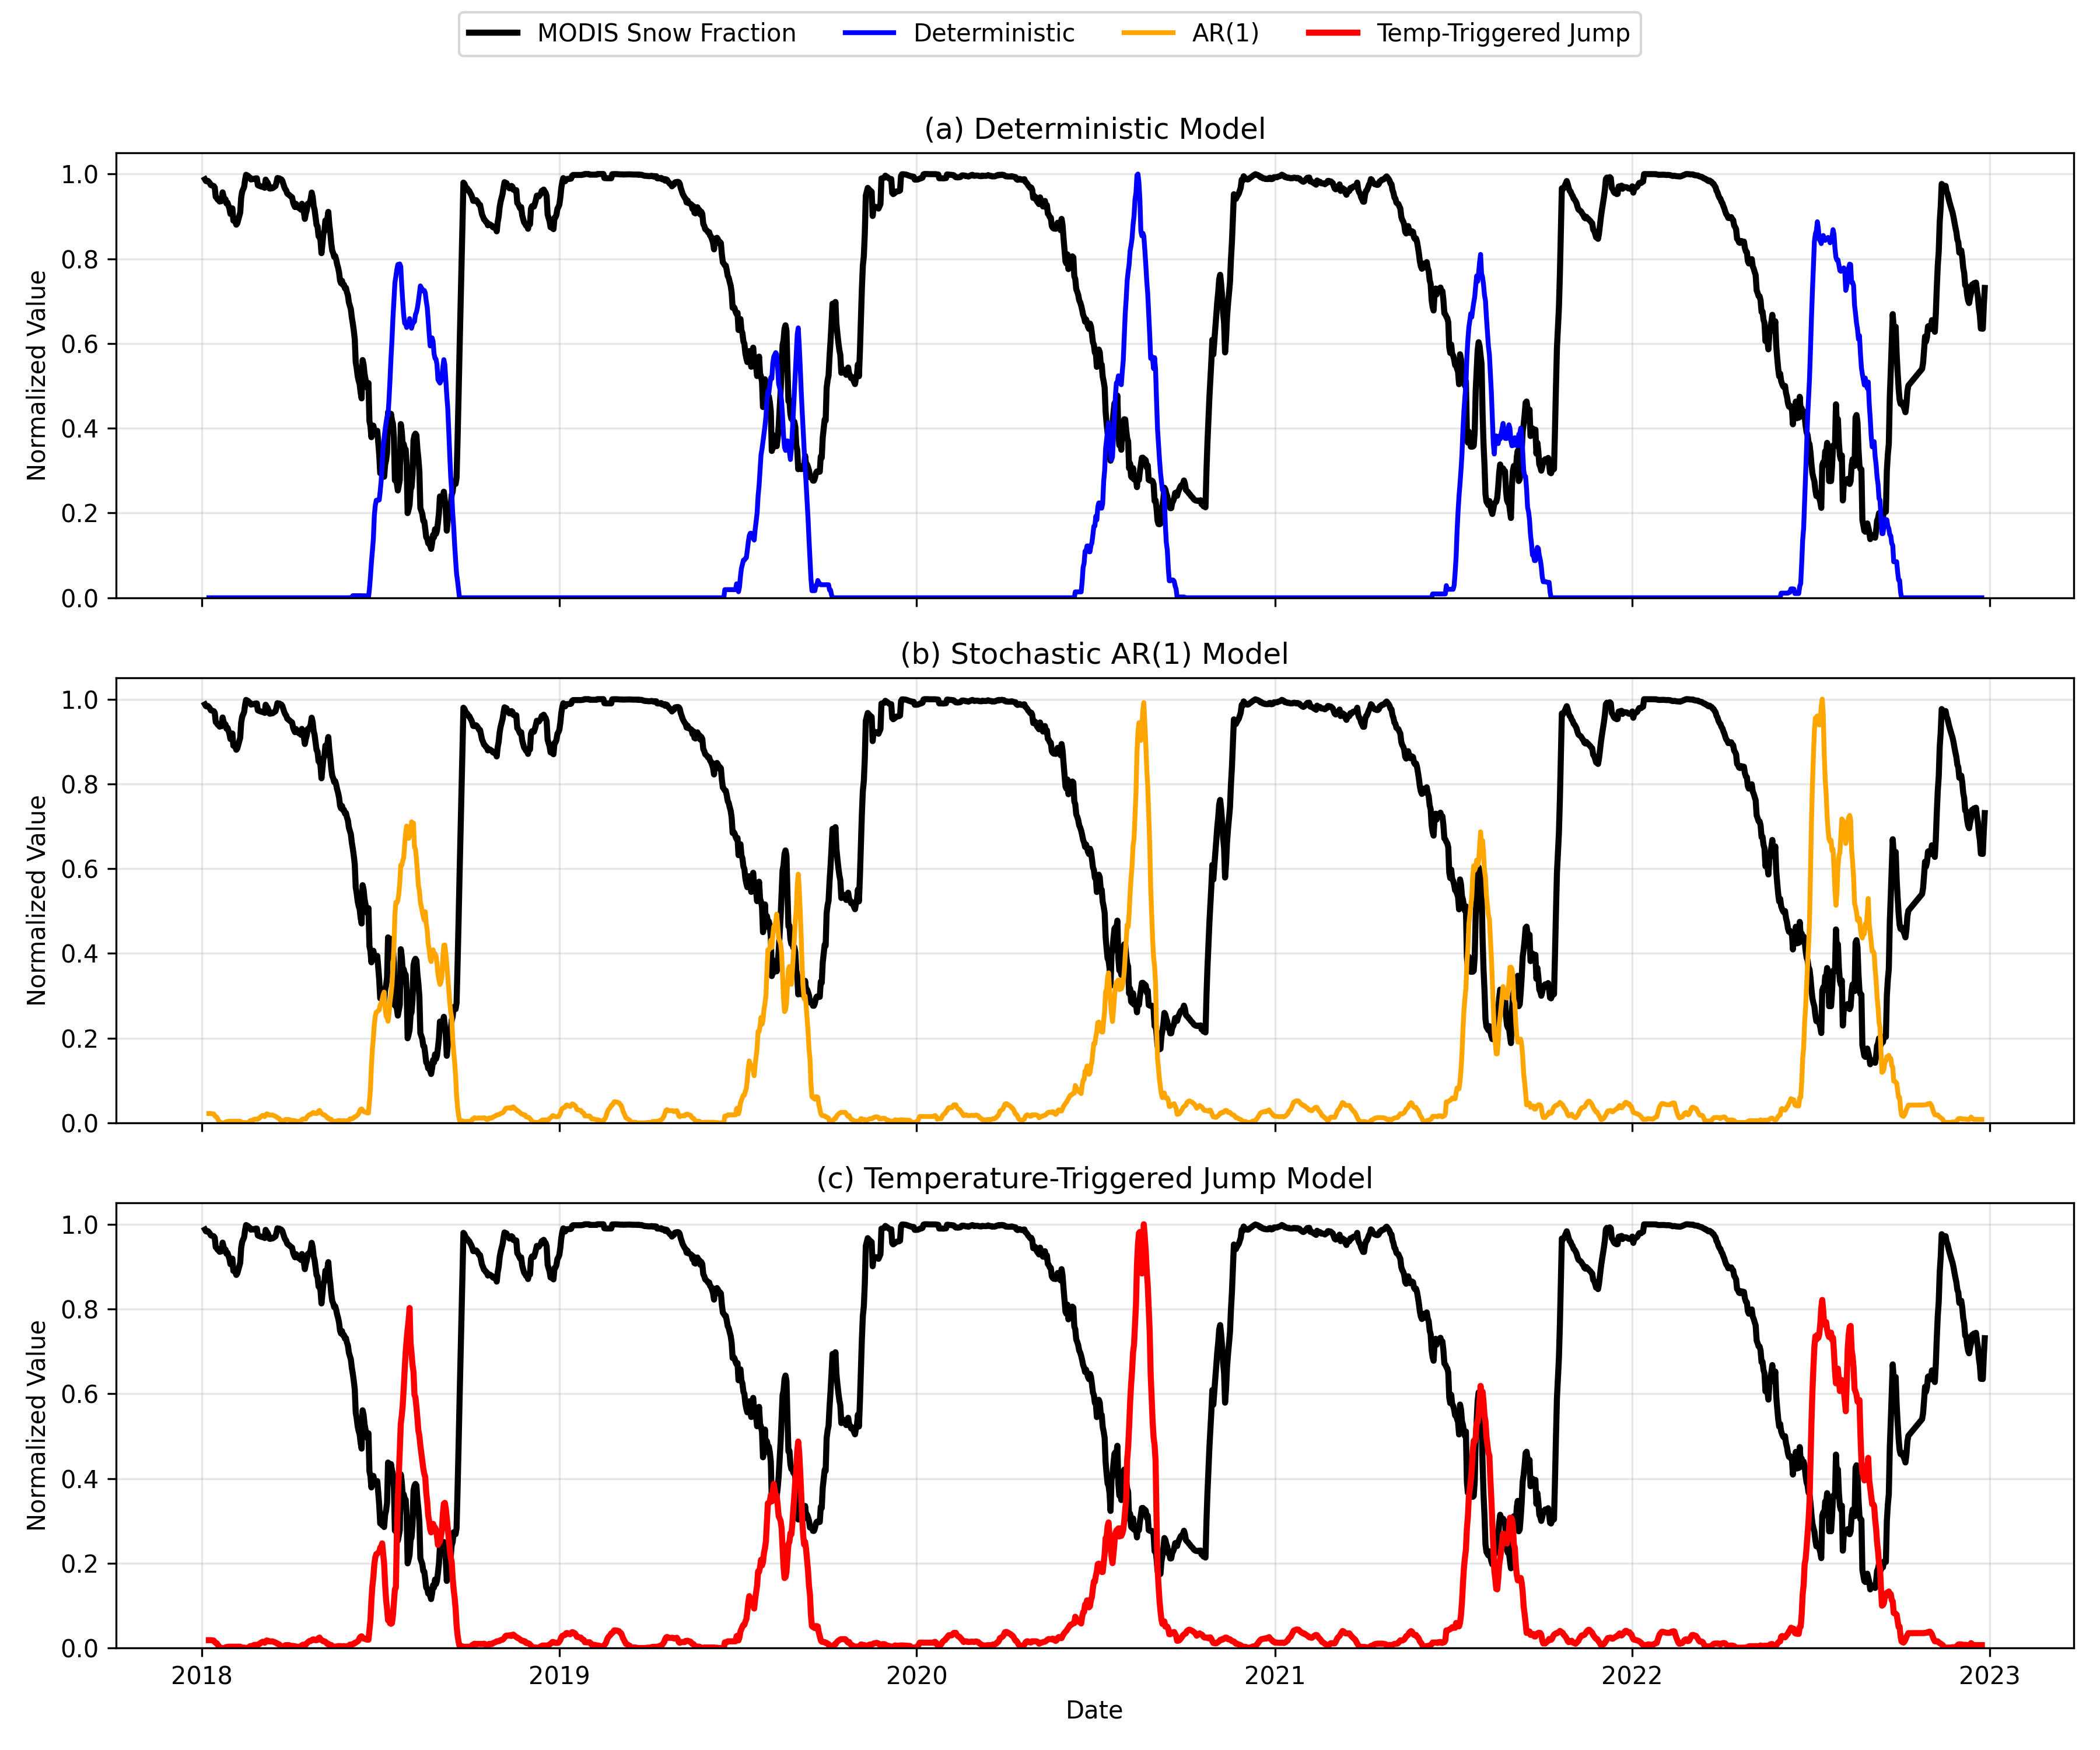
\includegraphics[width=\textwidth]{../outputs/figures/figure_validation_panels_final.png}
	\caption{Comparison between MODIS-derived basin-averaged snow fraction and normalized model melt outputs. The inverse relationship demonstrates consistency between modeled melt dynamics and observed snow depletion. Deterministic simulations capture seasonal trends, while stochastic models reproduce short-term variability.}
	\label{fig:validation}
\end{figure}

To evaluate the ability of the proposed models to represent real-world snow dynamics, model outputs were compared against satellite-derived snow cover observations from the MODIS dataset. Basin-averaged snow fraction time series were extracted and compared with normalized melt estimates from deterministic and stochastic models.

Figure~\ref{fig:validation} presents a direct comparison between MODIS-derived snow fraction and modeled melt dynamics across the study period. A clear inverse relationship is observed, with periods of decreasing snow cover corresponding to increased melt activity. This suggests that the model captures the fundamental physical linkage between temperature-driven melt and snow depletion.

The deterministic model exhibits the strongest temporal agreement with observed snow cover evolution, closely reproducing the seasonal accumulation--ablation cycle. In contrast, the stochastic models introduce additional variability, resulting in short-term fluctuations that deviate from the smooth seasonal signal but better represent intermittent melt behavior.

Quantitative evaluation supports these observations. The deterministic model shows the highest correlation with MODIS snow fraction ($r = -0.698$), indicating strong alignment with seasonal dynamics. The stochastic AR(1) and temperature-triggered jump models yield slightly lower correlations ($r = -0.662$ and $r = -0.633$, respectively), reflecting increased variability and reduced temporal smoothness.

However, stochastic models demonstrate improved magnitude representation, with lower root mean square error (RMSE). The AR(1) and jump models produce RMSE values of $0.755$ and $0.757$, respectively, compared to $0.772$ for the deterministic model. This indicates that stochastic formulations better capture variability and intensity of melt, despite reduced agreement in timing.

These results highlight a fundamental trade-off between temporal coherence and variability representation. Deterministic models are more effective in capturing large-scale seasonal patterns, whereas stochastic models better represent short-term variability and potential extreme melt behavior. This distinction is particularly relevant for applications involving hydrological risk assessment and uncertainty quantification.


	% =========================
	\section{Discussion}
	
	This study introduces a stochastic extension to the temperature-index snowmelt model, incorporating temporal persistence and state-dependent variability to better represent uncertainty in melt processes. The results demonstrate that while the deterministic formulation captures the dominant seasonal cycle, stochastic models provide additional insight into variability and extreme melt behavior.
	
	The deterministic model shows strong agreement with the seasonal evolution of snowmelt, reflecting its ability to represent large-scale temperature-driven processes. This is further supported by validation against MODIS snow cover, where the deterministic model achieves the highest correlation with observed snow depletion patterns ($r = -0.698$). This indicates that temperature alone is a strong predictor of basin-scale melt dynamics in the study region.
	
	However, deterministic models inherently lack the ability to represent variability arising from sub-grid heterogeneity, energy balance fluctuations, and measurement uncertainty. The stochastic AR(1) formulation addresses this limitation by introducing temporal persistence, resulting in smoother variability and improved representation of short-term fluctuations. The temperature-triggered jump model further extends this framework by capturing episodic melt events, producing intermittent spikes that resemble rapid melt pulses observed during warm conditions.
	
	Despite slightly lower correlation with MODIS observations ($r = -0.662$ for AR(1) and $r = -0.633$ for the jump model), stochastic models achieve lower RMSE values compared to the deterministic approach. This suggests that while stochastic formulations may reduce alignment in timing, they better represent the magnitude and variability of melt. These findings highlight a fundamental trade-off between temporal coherence and variability representation.
	
	The uncertainty analysis further reinforces the value of stochastic modeling. Ensemble simulations reveal a wide spread in melt outcomes, particularly during peak melt periods, indicating that deterministic models may underestimate uncertainty in hydrological predictions. This has important implications for water resource management and risk assessment, where understanding variability is as critical as estimating mean behavior.
	
	Nevertheless, several limitations must be acknowledged. The basin-aggregated approach neglects spatial heterogeneity associated with elevation gradients, aspect, and localized energy fluxes, which are particularly important in high-mountain environments such as the Himalaya. Additionally, the runoff model used in this study is highly simplified, relying on a linear relationship between melt and discharge, and does not account for routing processes, storage, or glacier contributions.
			
	Additionally, uncertainties associated with satellite-derived snow cover, including cloud contamination and classification errors, may influence validation accuracy and should be considered when interpreting results.
	
	
	This highlights the importance of moving beyond deterministic representations in snow hydrology, particularly for applications involving extremes, risk assessment, and climate variability.
	
\section{Conclusion}

This study develops a stochastic framework for snowmelt modeling by extending the traditional temperature-index approach to include temporal persistence and state-dependent variability. The proposed models generate probabilistic melt estimates, enabling representation of uncertainty and variability that are not captured by deterministic formulations.

Results indicate that the deterministic model effectively reproduces the seasonal structure of snowmelt, as confirmed by strong agreement with MODIS-derived snow cover observations. However, stochastic models provide improved representation of variability and melt intensity, as reflected in lower RMSE values and enhanced depiction of intermittent melt events.

The inclusion of stochastic processes allows the model to generate a distribution of possible melt outcomes, offering a more realistic characterization of uncertainty in snow-dominated hydrological systems. This is particularly relevant for applications involving risk assessment, forecasting, and climate sensitivity analysis.

Validation against satellite observations suggests that the model captures the fundamental relationship between temperature-driven melt and snow depletion. While deterministic models remain effective for representing large-scale seasonal behavior, stochastic extensions provide additional value by incorporating variability and uncertainty.

Overall, this study demonstrates that stochastic extensions of temperature-index models provide a meaningful advancement toward probabilistic hydrological modeling. By preserving simplicity while enhancing representation of variability and extremes, the proposed framework offers a practical pathway for improving snowmelt simulations in data-scarce mountainous environments. This approach is particularly relevant for applications involving hydrological risk, climate variability, and water resource planning under uncertainty.
	
	% =========================
\section{Future Work}

Several avenues exist for extending and improving the proposed modeling framework. A key priority is the incorporation of spatial heterogeneity through elevation-dependent modeling. Introducing temperature lapse rates and elevation band discretization would enable more realistic representation of snow accumulation and melt processes across complex terrain.

Integration of additional observational datasets offers significant potential for model improvement. In particular, MODIS snow cover data can be further utilized for quantitative calibration and data assimilation, rather than serving solely as a validation dataset. This would allow dynamic adjustment of model parameters based on observed snow conditions.

Future work should also focus on enhancing the runoff component of the model. Replacing the current linear runoff formulation with a physically based hydrological routing scheme would improve representation of streamflow dynamics, including storage, delay, and glacier contributions.

Parameter estimation remains another important area for development. Systematic calibration and sensitivity analysis of stochastic parameters, including persistence, variability scaling, and jump characteristics, would improve model robustness and interpretability. A key next step is formal calibration of stochastic parameters using observational constraints, enabling objective estimation of persistence and jump characteristics.

Finally, coupling the stochastic snowmelt framework with climate projections and high-resolution atmospheric models such as WRF would enable assessment of future changes in snow dynamics under different climate scenarios. This would provide valuable insights for water resource management and climate adaptation in snow-dominated regions.

These extensions would further strengthen the framework and enhance its applicability to both scientific research and operational hydrological modeling.

\section*{Data Availability}

All datasets used in this study are publicly available and reproducible. ERA5 reanalysis data were obtained from the European Centre for Medium-Range Weather Forecasts (ECMWF) Climate Data Store. The Shuttle Radar Topography Mission (SRTM) digital elevation model is publicly accessible through NASA data repositories.

All processed datasets, model outputs, and analysis scripts used in this study are available in a public GitHub repository:

\begin{center}
	\texttt{https://github.com/avinashparla/snowmelt-stochastic-model}
\end{center}

The repository includes:
\begin{itemize}
	\item Preprocessed basin-averaged temperature time series
	\item Deterministic and stochastic model outputs
	\item Monte Carlo simulation ensemble data
	\item Scripts for data processing, modeling, and figure generation
\end{itemize}

The code is provided to ensure full reproducibility of the results presented in this study.

	
	% =========================
	\bibliographystyle{plainnat}
	\bibliography{references}
	
\end{document}